\documentclass[tikz,border=2pt]{standalone}
\usepackage{pgfplots}
% \usepackage{pgf}
% \usepackage{tikz} % Required for drawing custom shapes
% \usetikzlibrary{calc}
% \usetikzlibrary{shapes,arrows,automata}
\usetikzlibrary{arrows.meta}

\begin{document}
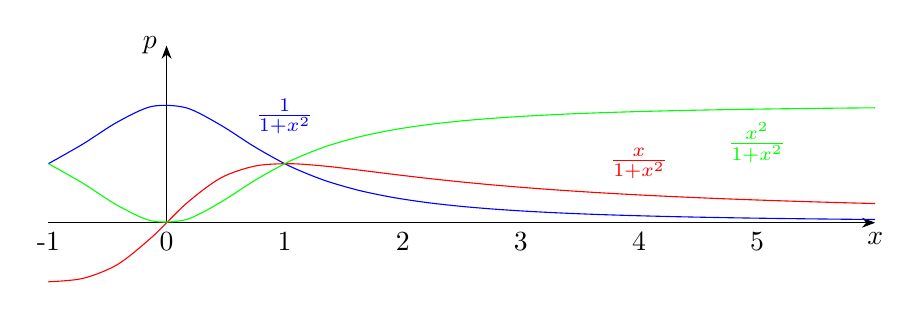
\begin{tikzpicture}[>=Stealth,scale=1.5]
\draw[<->](6,0)--(0,0)--(0,1.5);
\draw(0,0)--(-1,0);
\foreach \x in {-1,...,5}
    \node[below] at (\x,0) {\x};
\node[below] at (6,0) {$x$};
\node[left] at (0,1.5) {$p$};
% \draw[red,domain=-0.2:0.8] plot(\x,4*\x) node at (0.8,3.5){$y=4x$};
% \draw[blue,domain=-1:1] plot(\x,2*\x*\x) node at (1.1,2.2){$y=x^2$};
% \draw[cyan,domain=-1:2,smooth] plot(\x,{0.3*sin(4*\x r)}) node at (2.3,0.6){$y=0.3sin(4x)$};
\draw[blue,domain=-10:60,smooth] plot(\x/10,{1/(1+\x*\x/100)}) node at (1,0.9){$\frac{1}{1+x^2}$};
\draw[red,domain=-10:60,smooth] plot(\x/10,{\x/10/(1+\x*\x/100)}) node at (4,0.5){$\frac{x}{1+x^2}$};
\draw[green,domain=-10:60,smooth] plot(\x/10,{\x*\x/100/(1+\x*\x/100)}) node at (5,0.68){$\frac{x^2}{1+x^2}$};
\end{tikzpicture}
\end{document}